\documentclass[11pt,a4paper]{article}
\usepackage[T1]{fontenc}
\usepackage[utf8]{inputenc}
\usepackage{lmodern}
\usepackage[margin=1in]{geometry}
\usepackage{microtype}
\usepackage{amsmath,amssymb}
\usepackage{graphicx}
\usepackage{booktabs}
\usepackage{tabularx}
\usepackage{longtable}
\usepackage{array}
\usepackage[font=small,labelfont=bf]{caption}
\captionsetup[table]{position=top,skip=4pt}
\usepackage[authoryear,round]{natbib}
\usepackage{xr-hyper}
\externaldocument{supplement}
\usepackage[hidelinks]{hyperref}
\usepackage{xurl}
% archived copies of web sources, written by tools/archive_sources.py
\makeatletter
\newcommand{\archiveurl}[2]{\@namedef{arch@#1}{#2}}
\newcommand{\archived}[1]{\@ifundefined{arch@#1}{}{. Archived at \expandafter\url\expandafter{\csname arch@#1\endcsname}}}
\makeatother
\InputIfFileExists{archive_urls.tex}{}{}
\newcolumntype{L}{>{\raggedright\arraybackslash}X}
\newcolumntype{P}[1]{>{\raggedright\arraybackslash}p{#1}}
\setlength{\parskip}{0.35em}

\title{What the 50 Best Restaurants list can and cannot resolve:\\a sensitivity audit of its voting system}
\author{Samuele Lo Piano\\[2pt]
\small Faculty of Management and Economics, Gdansk University of Technology, Gdansk, Poland\\
\small Barcelona School of Management, Universitat Pompeu Fabra, Barcelona, Spain\\[6pt]
\small Correspondence: Faculty of Management and Economics, Gdansk University of Technology,\\
\small ul.\ Gabriela Narutowicza 11/12, 80-233 Gdansk, Poland\ifx\corremail\empty\else. E-mail: \corremail\fi\\[4pt]
\small Running head: Auditing a ranking built from votes}
\date{}
% the corresponding author's e-mail: set it here before compiling the submission PDF
\newcommand*{\corremail}{}

\begin{document}
\maketitle

\begin{abstract}
\noindent The 50 Best Restaurants ranks restaurants from the ballots of more than 1,100 experts in 28 regions, each naming ten restaurants. We use it to show how sensitivity auditing applies to vote-based rankings, separating what the published rules and lists establish, what holds under any distribution of votes, and what follows from scenarios for that distribution and from a generative ballot model. From the lists, places below the top ten move by a median of 9 to 18.5 positions between editions. With independent voters and whatever the distribution of votes, a fresh panel could keep at most 12 of the 49 adjacent pairs between the 51st and 100th places in order with probability 0.95, and a list without ties there would need the 51st restaurant to receive 49 more votes than the 100th. Under distributions consistent with the observed churn, a panel drawn again would put 10 to 12 different restaurants in the top 50. In the generative model, equal numbers of voters per region shape the geography of the list more than any other rule. The list measures visibility among a travelling, partly self-selected panel as much as quality, and three of its steps cannot be audited from outside.

\medskip\noindent\textbf{Keywords:} global sensitivity analysis, league tables, optimal transport, rankings, sensitivity auditing, voting rules
\end{abstract}

\section{Introduction}

Since 2002 the list now called The 50 Best Restaurants has ranked restaurants by the votes of an Academy of chefs, restaurateurs, food writers and travelling gourmets. The 2026 edition was revealed in Lima on 4 November 2026, two weeks after positions 51 to 100, and was the first under the new umbrella brand The 50 \citep{the50list2026,rebrand2026}. The list is consequential. A position moves bookings and careers, and national tourism agencies act as host partners of the ceremony, as the Peruvian promotion agency did for the 2026 edition \citep{the50partners2026,lima2026host}. The organiser presents the list as a snapshot of the opinions and experiences of its voters \citep{w50bvoting2026old}, yet publishes it as a strict ordering from 1 to 100 with no statement of how precise that ordering is.

A ranking is a model output. It rests on choices of who votes, how many votes each casts, where they may cast them, how votes are counted and how ties are broken, and on the randomness of which experts happen to sit on the panel in a given year. Sensitivity auditing \citep{saltelli2013latinorum,lopiano2022unpacking} extends sensitivity analysis to such instances of quantification by asking which assumptions are made, which of them matter, and whether the numbers are more precise than their inputs allow. The statistical literature on league tables reaches the same point from another direction: a ranking should come with a measure of its authority \citep{goldstein1996,hall2009}, and ties and near ties make that measure hard to obtain \citep{xie2009}.

Rankings built from votes are a class of quantification devices of their own. Reputation surveys of universities and hospitals, critics' polls and awards decided by panels share the structure of this list: a panel, a ballot, a counting rule and a published order, without the counts behind it. Sensitivity analysis of rankings has concentrated on rankings built from indicators, where weights and aggregation can be varied \citep{saisana2005,saisana2011}. A ranking built from votes offers no formula to perturb. Its inputs are ballots that are not released, and its precision depends on how many votes separate one position from the next. We use the 50 Best list to show how sensitivity auditing can be carried to such a device, by separating what the published rules and lists establish, what arithmetic and independent voters imply under any distribution of votes, and what needs a model of the votes (Section~\ref{sec:checklist}).

Section~\ref{sec:rules} sets out the rules as published, what they leave unsaid, and how they have changed, and Section~\ref{sec:checklist} introduces the seven rules of sensitivity auditing and the levels of evidence on which the rest of the audit rests. Section~\ref{sec:lists} measures what the published lists themselves reveal about the stability of positions. Section~\ref{sec:noise} asks how many positions a vote of this size can resolve, first under any distribution of votes and then under scenarios for it, and Section~\ref{sec:gsa} apportions the variability of the list to the organiser's rule choices, to what is unknown about the votes, and to the draw of the panel, with a global sensitivity analysis of a generative ballot model calibrated to the 2026 list. Section~\ref{sec:remedies} lists what would make the list more auditable, and Section~\ref{sec:conclusions} sets out the conclusions of the audit and what they imply for rankings built from votes.

\section{The voting system as published}\label{sec:rules}

Table~\ref{tab:rules} summarises the rules stated on the 2026 voting page and related pages of the organiser, and what they do not state. The Academy has more than 1,100 members in 28 regions, each headed by a Chair who recruits a set number of voters \citep{the50voting2026,the50academy2026}. The page gives no number per region, although the version it replaced in September 2026 stated 40 \citep{w50bvoting2026old}, in line with 1,120 voters in 28 regions in 2025 and 1,080 in 27 regions in 2022 \citep{upcoming2025,thenational2022}. Each voter names ten restaurants in order of preference, at most six in the home country, territory or Special Administrative Region (SAR), all eaten at within 18 months and documented by a proof of visit such as a booking confirmation, a receipt or a photograph. A restaurant needs votes from more than one country to be listed. The rules thereby define what the list measures: the restaurants that members of the panel have eaten at recently and choose to name, which depends on where they travel as well as on how good the restaurants are.

\begin{table}[t]
\caption{The 2026 voting rules as published, and what they leave unstated. Sources: \citet{the50voting2026,the50academy2026,the50faq2026,w50bvoting2026old,w50bdeloitte,asia50voting}.}
\label{tab:rules}
\small
\begin{tabularx}{\textwidth}{@{}P{2.6cm}LL@{}}
\toprule
Element & As published for 2026 & Not stated or inconsistent \\
\midrule
Academy & More than 1,100 members in 28 regions, each with a Chair who recruits a set number of voters; one third each of writers and critics, chefs and restaurateurs, and travelling gourmets; gender parity; at least 25\% renewed each year; members anonymous. & Number of voters per region (40 before the rebrand), selection criteria, and how Chairs are appointed and for how long. Chairs also advise on the strategy of the brand \citep{w50bfaq2025}. \\
Ballot & Ten restaurants in order of preference, at most six in the home country, territory or Special Administrative Region (SAR). & How the order is used. A 2026 version of the same page under the former domain stated 6 to 10 votes depending on the voter's ability to travel, with at most six in the home region. \\
Eligibility & Dined within 18 months, with proof of visit uploaded and not at off-site events; no financial interest; votes from more than one country; closed restaurants and former No.1s excluded. & Whether hosted or complimentary meals count, and how proofs are checked. \\
Counting & Not described on the 2026 global page. & Regional pages state that the order of preference decides ties and that the list is a simple computation of votes \citep{asia50voting}. \\
Adjustment & None on the 2026 page. & The adjudicator's page stated that a normalisation process may be applied to the voting data in the event of a significant variance between a region's share of votes and its representation in the list \citep{w50bdeloitte}. Trigger, method and use undefined. \\
Adjudication & Deloitte has full and independent access and performs procedures and checks. & Scope and findings of the procedures. \\
Positions 51--100 & Published two weeks before the top 50. & Same vote and adjudication according to earlier press releases \citep{restaurantnews2024}, not stated in 2026. \\
\bottomrule
\end{tabularx}
\end{table}

Three statements deserve emphasis because they bear directly on what the published order means. The first concerns ties. Before the rebrand, the regional voting pages said that the order of preference is used only when vote counts are equal, and the global page said the same in 2016 \citep{asia50voting,upcoming2016}. In 2007 ties were broken differently, by discounting votes from the restaurant's home region \citep{restaurant2007}. In 2015 two restaurants, Tickets and Borag\'o, were published as joint No.42, with no No.43 \citep{w50b2015pictures}, so exact ties do occur inside the top 50. The 2026 global page says only that choices are submitted in order of preference. The second concerns the regional normalisation. Before the rebrand, the adjudicator's page and the voting page for the global list, and the 2026 rules of the Latin American list, stated that Deloitte will apply a ``normalisation process to the voting data'' when a region's share of votes and its share of the list diverge significantly \citep{w50bdeloitte,w50bvoting2026old,latam50voting}. The regional pages that carried the clause also described their lists as a simple computation of votes \citep{asia50voting,latam50voting}. Neither the size of variance that triggers the step, nor the operation, nor the editions in which it was applied are published. The third concerns the ballot. A 2026 version of the global page under the former domain described a variable ballot of six to ten votes depending on the voter's ability to travel internationally \citep{w50bvoting2026old}, while the current page states ten votes. Which rule produced the 2026 list is therefore not clear from the organiser's own pages. The voting pages published after the rebrand mention neither the number of voters per region, nor the variable ballot, nor the normalisation.

\begin{table}[t]
\caption{Rule changes and discretionary decisions that affect the comparability of editions.}
\label{tab:drift}
\small
\begin{tabularx}{\textwidth}{@{}P{1.7cm}L@{}}
\toprule
Edition & Change \\
\midrule
2007 & 22 voting regions; ties broken by discounting home-region votes \citep{restaurant2007}. \\
2016 & Seven votes per voter, at least three outside the home region; order of preference used for ties \citep{upcoming2016}. \\
2019 & Ten votes per voter in 26 regions \citep{fwg2019}; former No.1s made ineligible (Best of the Best); the extended list lengthened from 100 to 120 places to mark the main sponsor's 120th anniversary \citep{inkl2019}. \\
2021 & Noma, a former No.1, eligible again as a new restaurant after relocation and a change of concept and ownership, and named No.1 \citep{sansom2021noma}. \\
2022 & 1,080 voters in 27 regions \citep{thenational2022}; Russian restaurants excluded by the organiser \citep{falstaff2022}. \\
2025 & 1,120 voters in 28 regions \citep{upcoming2025}. \\
2026 & More than 1,100 voters; home limit stated per country, territory or SAR; proof of visit required; renamed The 50 Best Restaurants; host destination moved from Abu Dhabi to Lima \citep{the50voting2026,lima2026host}. \\
\bottomrule
\end{tabularx}
\end{table}

The rules have changed in almost every dimension (Table~\ref{tab:drift}). The number of regions grew from 22 to 28, the ballot from seven to ten votes, and the out-of-region quota was redefined. Some decisions were made outside the vote altogether: former winners were retired, one of them was readmitted as a new restaurant, Russian restaurants were excluded, and the length of the extended list was set once by a sponsor's anniversary. Each of these is defensible on its own terms, but together they mean that a restaurant's rise or fall between editions mixes changes in votes with changes in rules.

\section{Auditing a ranking built from votes}\label{sec:checklist}

Sensitivity auditing \citep{saltelli2013latinorum,lopiano2022unpacking} reads an instance of quantification against seven rules. They ask whether the numbers are used rhetorically, which assumptions they rest on, whether the inputs can support the outputs, which assumptions matter most, whether the procedure is transparent, whether the numbers answer the right question, and whether their uncertainty has been analysed. The published rules of Section~\ref{sec:rules} answer some of these questions, and the others need the quantitative analysis of Sections~\ref{sec:lists} to~\ref{sec:gsa}. Section~\ref{sec:conclusions} reads the findings against all seven rules (Table~\ref{tab:checklist}).

The seven rules say where to look but not how strong each finding is. For a ranking built from unpublished votes we separate four levels of evidence, each adding assumptions to the one before (Table~\ref{tab:evidence}). The published rules and lists establish facts without any model. Arithmetic on integer counts, and the variability of a panel of independent voters, give limits that hold whatever the distribution of votes. Scenarios for that distribution, constrained by the observed churn, give magnitudes. A generative model of ballots, calibrated to the published list, apportions the variability of the list among the rules. Each conclusion of the audit is labelled by the level it needs, so that a reader who rejects a model keeps the conclusions that do not rest on it. The same four levels apply to any ranking that aggregates the ballots of a panel.

\begin{table}[t]
\caption{Levels of evidence in the audit, what each assumes in addition to the one before, and what it can establish.}
\label{tab:evidence}
\small
\begin{tabularx}{\textwidth}{@{}P{3.1cm}P{4.0cm}L@{}}
\toprule
Level & Assumptions added & What it can establish \\
\midrule
1. Published rules and lists (Sections~\ref{sec:rules} and~\ref{sec:lists}) & None & What the rules state and leave undefined, how they have changed, and how stable positions have been between editions. \\
2. Any vote curve (Section~\ref{sec:bounds}) & Integer counts from at most 11,200 votes. For the second result, expected counts in the published order and voters who choose independently, so that counts are independent binomials. & Limits on how many adjacent positions the vote can separate, whatever the distribution of votes. \\
3. Vote-curve scenarios (Section~\ref{sec:scenarios}) & Power-law expected votes, constrained by the observed churn. & The extent of ties, rank intervals, and how much of the observed movement the renewal of the panel alone produces. \\
4. Generative ballot model (Section~\ref{sec:gsa}) & Plackett--Luce ballots with home bias, calibrated to the 2026 order, and unlisted restaurants spread evenly over regions. & How the variability of the list divides among the rules, the vote curve and the draw of the panel. \\
\bottomrule
\end{tabularx}
\end{table}

\section{What the published lists show}\label{sec:lists}

We assembled the published lists of 2002 to 2026, positions 1 to 50 in every edition and positions 1 to 100 in the seven editions from 2019 to 2026 (no list was published in 2020, and the 2019 extended list ran to No.120). The lists of 2002 to 2025 come from the organiser's own archive of past lists \citep{the50archive}, which gives positions 1 to 50 up to 2022 and 1 to 100 from 2023. The extended lists of 2019, 2021 and 2022, which the archive does not hold, come from press coverage of the organiser's releases, each checked against a second source, and the 2026 list from the organiser's pages (Appendix~\ref{app:data}). The archive departs from the organiser's own announcements at four positions in three editions, which we correct. As a check of the whole assembly, the 2023 extended list was reported with each restaurant's change since 2022, and our panel reproduces all 50 of those changes exactly. Everything in this section follows from the published lists, without a model.

\begin{figure}[t]
\centering
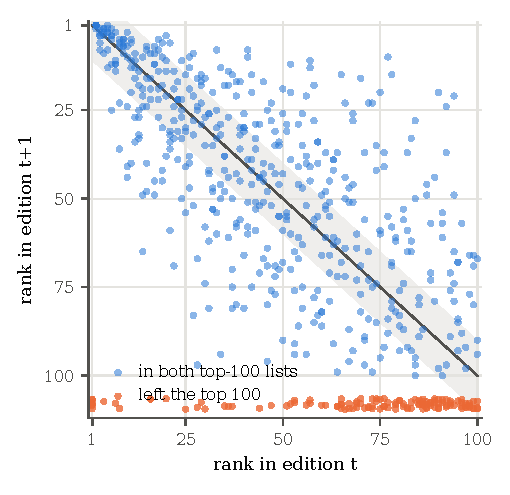
\includegraphics[width=0.55\textwidth]{figures/fig_pairs.pdf}
\caption{Rank in one edition against rank in the next, 2019 to 2026, pooled over six transitions (600 restaurant-transitions). Blue: restaurants in both top-100 lists. Orange: restaurants that left the top 100, including retired No.1s and closures. The shaded band is within ten places of the previous rank.}
\label{fig:pairs}
\par\smallskip{\footnotesize Alt text: Scatter plot of each restaurant's rank in one edition against its rank in the next, for the six transitions from 2019 to 2026. Points stay close to the diagonal in the top ten and spread widely below rank 25, and many restaurants ranked below 50 leave the next top 100.\par}
\end{figure}

Figure~\ref{fig:pairs} shows the 600 transitions between consecutive top-100 lists from 2019 to 2026. Among the restaurants present in both lists, the rank correlation between editions ranges from 0.63 to 0.79 (median 0.69). Table~\ref{tab:bands} summarises the movements by band of the earlier rank, after removing the mechanical gain of one place that every restaurant receives when the previous No.1 is retired. Movements grow quickly below the top ten. Half of the restaurants ranked 26 to 50 moved by 13 places or more, and one in ten by 34 places or more. In the lower half of the list the median movement is 16 to 19 places, and almost half of the restaurants ranked 76 to 100 were not in the next top 100. Across the halves of the list, 18\% of the restaurants in a top 50 fell to positions 51 to 100 in the next edition, and 21\% of those in positions 51 to 100 rose into the top 50.

\begin{table}[t]
\caption{Movements between consecutive editions, 2019 to 2026, by band of the earlier rank, with the retired No.1 removed and the resulting one-place gain discounted.}
\label{tab:bands}
\small
\begin{tabular*}{\textwidth}{@{\extracolsep{\fill}}lrrrrr@{}}
\toprule
Band of earlier rank & 1--10 & 11--25 & 26--50 & 51--75 & 76--100 \\
\midrule
Restaurant-transitions & 60 & 90 & 150 & 150 & 144 \\
Left the next top 100 (\%) & 5 & 4 & 6 & 24 & 45 \\
Median absolute change, those remaining & 2 & 9 & 13 & 18.5 & 16 \\
90th percentile of absolute change & 15 & 27 & 34 & 39 & 45 \\
Moved 10 places or more (\%) & 14 & 48 & 61 & 73 & 67 \\
\bottomrule
\end{tabular*}
\end{table}

Exits from the top of the list are rare and mostly have causes outside the vote. Of the 21 restaurants that were in a top 50 and absent from the next top 100 between 2019 and 2026, six were No.1s retired under the Best of the Best rule and two were the Russian restaurants excluded in 2022. Of the five 2026 cases, Lido 84 closed in March 2026, Table by Bruno Verjus announced its closure for the end of 2026, and S\'ezanne lost the chef who had opened it \citep{lido84closure,tableclosure,sezanne2026}.

The retirement rule has changed what the No.1 position means (Table~\ref{tab:succession}). Before 2019, the No.1 was retained in six of 16 transitions, and when it changed hands, the previous No.2 took it in seven of ten cases and the previous No.3 in the other three. Since 2019 the previous No.1 is always retired, and in six of the seven editions the new No.1 was the highest-placed eligible restaurant of the previous edition. The exception is Maido, No.5 in 2024 and No.1 in 2025, while Asador Etxebarri stayed at No.2 and was named No.1 in 2026. In practice, the title is largely settled a year in advance, when the runner-up is chosen.

\begin{table}[t]
\caption{The No.1 since the Best of the Best rule, and its rank in the previous edition.}
\label{tab:succession}
\small
\begin{tabular*}{\textwidth}{@{\extracolsep{\fill}}llrl@{}}
\toprule
Edition & No.1 & Previous rank & Highest eligible restaurant of the previous edition \\
\midrule
2019 & Mirazur & 3 & Mirazur (Nos.1 and 2 of 2018 already former No.1s) \\
2021 & Noma & 2 & Noma \\
2022 & Geranium & 2 & Geranium \\
2023 & Central & 2 & Central \\
2024 & Disfrutar & 2 & Disfrutar \\
2025 & Maido & 5 & Asador Etxebarri \\
2026 & Asador Etxebarri & 2 & Asador Etxebarri \\
\bottomrule
\end{tabular*}
\end{table}

Over the longer run, the rank correlation among restaurants that stayed in consecutive top-50 lists has a median of 0.71 since 2010. The 2025 to 2026 transition has the lowest such correlation since the 2003 to 2004 transition: 16 of the 2025 top 50 left the top 50, and the correlation among the 34 that stayed was 0.49.

\section{How many positions can the vote resolve?}\label{sec:noise}

Vote counts are not published, so the precision of the 2026 list cannot be computed directly. This section proceeds in two steps that rest on different assumptions. The first gives limits that hold whatever the distribution of votes, using only the fact that counts are integers from a fixed number of ballots and, for the second limit, that voters choose independently. The second step assumes a distribution of votes. That distribution is unknown, and the scenarios we use are constrained only by the year-on-year churn observed in Section~\ref{sec:lists}. Every figure in the second step, and in Section~\ref{sec:gsa}, inherits this assumption.

\subsection{What holds under any vote curve}\label{sec:bounds}

Let $v_r$ be the number of votes of the restaurant published at position $r$. With $N = 1{,}120$ voters casting at most $L = 10$ votes, all counts add up to at most $NL = 11{,}200$. The first result is arithmetic. Between positions $a$ and $b$ the counts can fall by one vote or more at most $v_a - v_b$ times, so at least $(b - a) - (v_a - v_b)$ of the $b - a$ adjacent pairs are tied. A list with no tie between No.51 and No.100 needs No.51 to have at least 49 more votes than No.100, and since the 51 restaurants at the top share at most 11,200 votes, No.51 cannot have more than 219.

The second result takes the published order to be the order of expected votes, which is what keeping that order means, and adds one assumption, that voters choose independently of one another and that the count of one restaurant says nothing about the count of another, so that the count of a restaurant expected to receive $\mu$ votes is binomial with mean $\mu$. A fresh panel then reverses two restaurants expected at $\mu_a > \mu_b$ with a probability that depends only on $\mu_a$ and $\mu_b$, counting a tie as a reversal in half the cases. For an adjacent pair to be kept in order with probability 0.95, the upper restaurant must expect at least $g(\mu_b)$ votes, where $g$ grows with $\mu_b$. Starting from zero, a run of $r$ such pairs therefore needs expected counts of at least $c_1 < c_2 < \dots < c_r$, with $c_1 = g(0) = 2.3$, $c_2 = g(c_1) = 7.3$, $c_3 = 14.9$ and so on, and every restaurant above the run needs at least $c_r$. Comparing these minimal costs with the 11,200 available votes bounds the number of pairs that any vote curve can resolve (Table~\ref{tab:bounds}). The bound is generous, since it gives every vote to the listed restaurants and lets the lowest of them have none.

\begin{table}[t]
\caption{Most adjacent pairs of positions that a fresh panel could keep in order with the stated probability, under any distribution of 11,200 votes among restaurants and with voters choosing independently.}
\label{tab:bounds}
\small
\begin{tabular*}{\textwidth}{@{\extracolsep{\fill}}lrrrr@{}}
\toprule
 & & \multicolumn{3}{c}{Kept in order with probability} \\
\cmidrule(l){3-5}
Positions & Adjacent pairs & 0.95 & 0.90 & 0.75 \\
\midrule
\csname @@input\endcsname table_bounds.tex 
\bottomrule
\end{tabular*}
\end{table}

Whatever the distribution of votes, at most 12 of the 49 adjacent pairs between No.51 and No.100, and at most 16 of the 24 between No.26 and No.50, could be kept in order with probability 0.95. Even at 0.75, a level at which one order in four would be reversed, no more than 28 of the 49 pairs in the lower half qualify. The top 25 is different. Nothing in these limits prevents its 24 adjacent pairs from being resolved, so whether they are depends on the distribution of votes, which is what the next subsection assumes. These limits are the sharpest statement the audit can make about the published order, because they need no vote curve and only the simplest model of ballots. Departures from that model work in both directions. Panels recruited through the same networks make counts more variable, and a ballot of fixed length makes the counts of two restaurants slightly negatively correlated, both of which strengthen the limits. Restaurants named on the same trips have positively associated counts, and a fixed number of voters per region makes the count of a restaurant that draws its votes from its own region less variable than a binomial count, both of which weaken them. The second effect can be bounded. If every restaurant drew 60\% of its expected votes from the 40 voters of its own region, at most 14 of the 49 pairs between No.51 and No.100 could be kept in order with probability 0.95, and at most 18 if it drew all the votes its region can give, one from every voter there.

\subsection{Scenarios for the vote curve}\label{sec:scenarios}

To go further we need a distribution of votes, and we use the published churn to rule out distributions that are inconsistent with it. Let $\mu_r$ be the expected number of votes for the restaurant at position $r$, with $\sum_r \mu_r = N L$ for $N = 1{,}120$ voters casting $L = 10$ votes. We take $\mu_r = v_1 r^{-\alpha}$, continued below No.100 until all votes are used, and index scenarios by the expected votes of No.100, $v_{100} \in \{12, 20, 28\}$, and the ratio $v_1 / v_{100} \in \{5, 8, 12\}$. Scenario M8, for instance, has 160 expected votes for No.1, 27 for No.50 and 20 for No.100, with 31\% of all votes on the top 100. The nine scenarios put between 16\% and 50\% of all votes on the top 100. Each voter includes restaurant $r$ with probability $\mu_r/N$, so a panel drawn again yields binomial counts. This is the variability of a panel of independent voters drawn from the same population. Correlated recruitment, such as panels assembled through the same networks, would add to it.

\begin{table}[t]
\caption{Share of adjacent positions with equal vote counts in simulated editions, by part of the list, for the nine vote-distribution scenarios (L, M, H: $v_{100}$ = 12, 20, 28 votes; 5, 8, 12: ratio $v_1/v_{100}$).}
\label{tab:ties}
\small
\begin{tabular*}{\textwidth}{@{\extracolsep{\fill}}lrrrrrrrrr@{}}
\toprule
Positions & L5 & L8 & L12 & M5 & M8 & M12 & H5 & H8 & H12 \\
\midrule
1--25 & 0.44 & 0.33 & 0.26 & 0.32 & 0.22 & 0.17 & 0.24 & 0.18 & 0.13 \\
26--50 & 0.84 & 0.77 & 0.71 & 0.74 & 0.65 & 0.57 & 0.65 & 0.54 & 0.47 \\
51--100 & 0.93 & 0.91 & 0.89 & 0.89 & 0.86 & 0.82 & 0.85 & 0.80 & 0.76 \\
Distinct counts in 51--100 & 4 & 5 & 6 & 6 & 8 & 10 & 8 & 11 & 13 \\
\bottomrule
\end{tabular*}
\end{table}

The first consequence is the extent of ties (Table~\ref{tab:ties}). In every scenario, between 76\% and 93\% of adjacent pairs from No.51 to No.100 have the same number of votes, and the 50 positions share four to 13 distinct counts. Between No.26 and No.50 the share is 47\% to 84\%. These shares follow from the arithmetic of Section~\ref{sec:bounds}: in the nine scenarios No.51 expects only 3 to 12 more votes than No.100, which leaves room for about that many changes of count across 49 adjacent pairs. The order within these groups is set by the tie-break, which the 2026 global rules do not describe.

\begin{figure}[t]
\centering
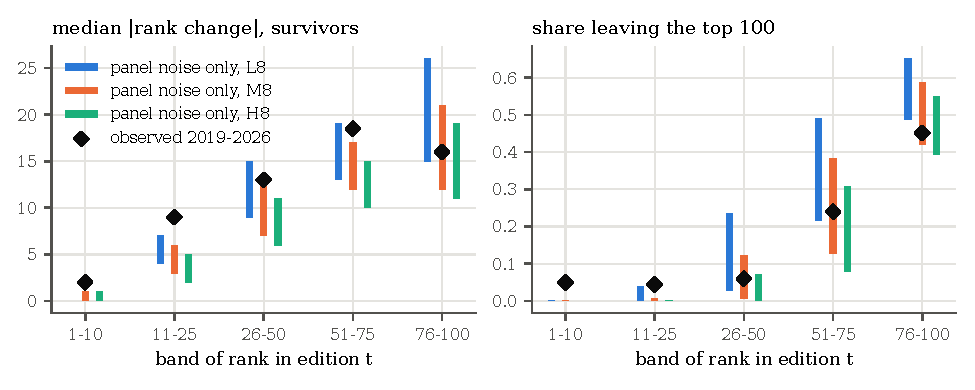
\includegraphics[width=\textwidth]{figures/fig_churn.pdf}
\caption{Year-on-year movements that panel noise alone would produce if no restaurant changed, against the movements observed from 2019 to 2026 (black diamonds, with the retired No.1 removed). Each bar spans two bounds. The lower end keeps the ballots of the 75\% of voters who stay and redraws the renewed quarter, and the upper end redraws all ballots. Scenarios L8, M8 and H8 as in Table~\ref{tab:ties}. Left: median absolute change among restaurants in both top-100 lists. Right: share leaving the top 100.}
\label{fig:churn}
\par\smallskip{\footnotesize Alt text: Two bar charts by band of the earlier rank, for three vote-curve scenarios. Bars show the range of median absolute rank change (left) and of the share of restaurants leaving the top 100 (right) that panel noise alone produces, and black diamonds show the observed values. Below rank 25 the observed values lie inside or at the edge of the bars.\par}
\end{figure}

The second consequence is the width of rank intervals (Figure~\ref{fig:intervals} in Section~\ref{sec:gsa}, dashed lines). In scenario M8 the 90\% interval of a restaurant whose expected position is No.10 runs from 7 to 17, No.25 from 16 to 54, No.50 from 29 to 123, and No.100 from 54 to 302. In H8, with 40\% more votes on the top 100, the corresponding intervals are 7 to 16, 17 to 45, 32 to 106 and 59 to 241. A panel of the same size drawn independently would keep on average 42 to 43 of the expected top 50 in the top 50. The published list is itself the result of one panel, and two panels drawn independently share only 38 to 40 of their top 50, so a panel drawn again would put 10 to 12 different restaurants in the top 50.

The third consequence concerns the year-on-year changes that are reported every edition as risers and fallers. Figure~\ref{fig:churn} compares the observed movements with those that panel noise alone would produce if no restaurant changed. The two bounds bracket the overlap of consecutive panels: one keeps the ballots of the 75\% of voters who stay, the other redraws all ballots, as the shift of the 18-month window would partly do. Scenario L5 predicts more exits than were observed in every band below No.25, even at the lower bound, and can be ruled out. L8 and M5 do so only for positions 76 to 100, and by less than the sampling error of the observed share (four percentage points), so they remain plausible. For the plausible scenarios, the observed movements in positions 26 to 100 lie inside or at the edge of the band that pure panel noise produces, both in median movement and in the share leaving the top 100. Only in the top 25 do observed movements exceed noise, which means that real changes in standing are detectable there. Applying the noise bands of scenario M8 to the 2025 to 2026 transition, and comparing each restaurant in both lists with unchanged restaurants that also stay in the top 100, 19 of the 82 moved by more than the upper noise bound allows at the 90\% level. With no change at all, about eight would fall outside by chance, so the excess points to real changes in standing without singling out each of them. The largest are the movements that the vote certifies, such as Don Julio falling from No.10 to No.44, Kadeau rising from No.41 to No.8, and Al Gatto Verde and Meet the Bund rising from the low 90s into the top 25. The remaining 63 are compatible with no change at all under this bound, and 54 under the stricter one that keeps the ballots of returning voters.

\section{Sensitivity of the list to the voting rules}\label{sec:gsa}

This section adds a model of how voters fill their ballots, the fourth level of Table~\ref{tab:evidence}, and its conclusions hold only as far as that model does. The binomial model says how precise the list is under its own rules. To ask how much the rules themselves shape the list, we need a model of ballots. We use a random-utility model in which voter $i$ from region $g(i)$ values restaurant $j$ at $u_{ij} = \theta_j + h\,\mathbb{1}[g(j) = g(i)] + \varepsilon_{ij}$, with independent Gumbel errors, so that each ballot is a Plackett--Luce draw \citep{luce1959,plackett1975}. A ballot holds the $L$ restaurants with the highest utility subject to at most $C$ in the voter's home region, in order of preference, so that positional counting rules can be applied to it. The candidates are the 2026 top 100, in their regions, and the restaurants below No.100 implied by the vote-curve scenario, spread evenly over the 28 regions. For each world, defined by a vote curve and a home bias $h$, the appeals $\theta_j$ are calibrated so that under the published rules the expected votes follow the scenario curve, which makes the published 2026 order the expected order of the model. The calibration reproduces the target votes within 1.7\% to 3.4\% on average (Monte Carlo error of the check included), with a rank correlation of 0.98 or more between expected and published order. With $h = 3$ about 37\% to 40\% of votes go to the home region, and with $h = 5$ about 57\% to 60\%, where the cap of six binds (72\% to 82\% would go home without it).

\begin{table}[t]
\caption{Factors of the global sensitivity analysis. Published rules in bold. All levels are crossed (432 cells), with 16 independently drawn panels per cell (6,912 simulated editions).}
\label{tab:factors}
\small
\begin{tabularx}{\textwidth}{@{}P{3.3cm}P{5.4cm}L@{}}
\toprule
Factor & Levels & Meaning \\
\midrule
Counting rule & \textbf{approval count}, Borda, Dowdall & Each vote counts one; positions weighted $L, L-1, \dots, 1$; positions weighted $1, 1/2, \dots, 1/L$ \\
Ballot length & 7, \textbf{10} & Votes per voter before and after the late 2010s \\
Home cap & 30\%, \textbf{60\%}, 100\% of the ballot & At most 3, 6 or 10 of 10 votes at home \\
Voters per region & \textbf{40 in every region}, by supply & Equal, or proportional to one plus the region's places in the 2026 top 100 (floor of 10) \\
Tie-break & \textbf{order of preference}, random & Among equal approval counts \\
Vote curve & L8, M8, H8 & Expected votes as in Section~\ref{sec:noise} \\
Home bias & $h = 3$, $h = 5$ & Moderate or strong preference for the home region \\
Panel draw & 16 replicates & Which voters sit on the panel \\
\bottomrule
\end{tabularx}
\end{table}

The design crosses five rule factors with two factors describing what is unknown about the votes (Table~\ref{tab:factors}). Every simulated edition is summarised by six features: the rank correlation of the 2026 top 100 with their published order, the number of the published top 50 and top 10 that remain there, the mean displacement of the published 51 to 100 (with simulated positions below No.200 counted as No.200), the number of Academy regions represented in the top 50, and the number of European restaurants in the top 50. Because the design is a full factorial, first-order and total Sobol' indices \citep{sobol2001} are exact functions of the cell means. With $m(\mathbf{x})$ the mean of a cell and $s^2(\mathbf{x})$ its within-cell variance over panels, $S_i = \mathrm{Var}(E[m \mid x_i])/\mathrm{Var}(Y)$, $S_{Ti} = E[\mathrm{Var}(m \mid \mathbf{x}_{\sim i})]/\mathrm{Var}(Y)$ after subtracting the panel noise left in the cell means, and the share of the panel draw is $E[s^2]/\mathrm{Var}(Y)$. We also report the optimal-transport index of \citet{borgonovo2025ot}, $\iota_i = E[W_2^2(P_Y, P_{Y \mid x_i})]/(2\,\mathrm{Var}\,Y)$, computed with the exact one-dimensional Wasserstein distance, and a dummy factor gives its null level (Section~\ref{app:ot} of the supplementary material). Intervals are 95\% jackknife intervals that leave out one of the 16 panels of every cell at a time.

\begin{figure}[t]
\centering
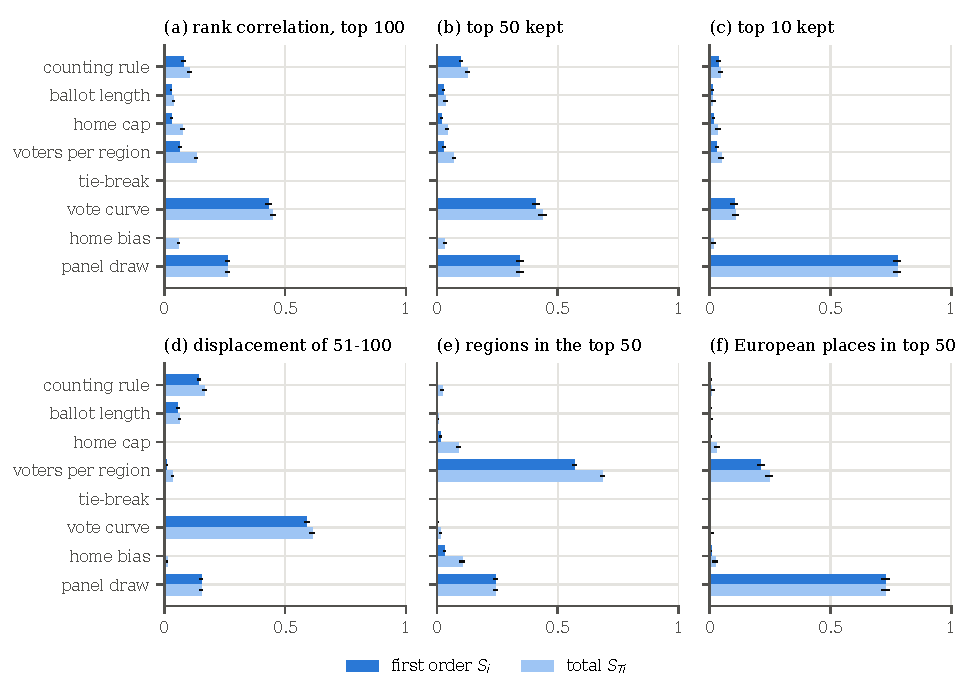
\includegraphics[width=\textwidth]{figures/fig_indices.pdf}
\caption{First-order and total Sobol' indices of six features of the simulated list, with 95\% jackknife intervals. Panel draw: share of variance due to the panel within each cell. Displacement: positions below No.200 counted as No.200.}
\label{fig:indices}
\par\smallskip{\footnotesize Alt text: Six horizontal bar charts, one per feature of the simulated list, with first-order and total Sobol' indices for the five voting rules, the vote curve, the home bias and the panel draw. The vote curve and the panel draw carry most of the variance of the rank correlation, the top-50 overlap and the displacement, the panel draw that of the top ten, and the allocation of voters that of the regions in the top 50.\par}
\end{figure}

Figure~\ref{fig:indices} shows the indices. For the agreement of the list with its published order, measured by the rank correlation of the top 100, the share of the published top 50 kept and the displacement of positions 51 to 100, the two largest sources of variance are the vote curve ($S_i$ = 0.43, 0.41 and 0.59) and the panel draw (0.26, 0.34 and 0.15). The vote curve matters because it fixes how many votes separate positions, which is exactly what the organiser does not publish. Among the rules, the counting rule has the largest effect ($S_i$ = 0.08, 0.10 and 0.14), followed by the allocation of voters, ballot length and the home cap, each below 0.07 at first order. The tie-break has no measurable effect, because the order of preference among tied restaurants carries little information beyond what the counts already contain. The top ten is dominated by the panel draw (0.78). The geography of the list responds to one rule. The allocation of voters explains 57\% of the variance in the number of regions represented in the top 50 (69\% with interactions) and 21\% of the variance in the number of European restaurants, the rest being mostly panel noise. Because voters name restaurants they have eaten at, the allocation of voters decides whose visits the list counts, which is a choice about visibility rather than about quality.

\begin{table}[t]
\caption{Mean features of the simulated list when one rule departs from the published rules and the others stay at their published values, averaged over the six worlds and 16 panels. Published rules in the first row of each block. Spearman: rank correlation of the 2026 top 100 with their published order. Top 50 and Top 10: published restaurants that remain there. Displ.: mean displacement of the published 51--100, with positions below No.200 counted as No.200. Regions: Academy regions in the top 50. Europe: European restaurants in the top 50.}
\label{tab:effects}
\small
\begin{tabular*}{\textwidth}{@{\extracolsep{\fill}}llrrrrrr@{}}
\toprule
Rule & Level & Spearman & Top 50 & Top 10 & Displ. & Regions & Europe \\
\midrule
\csname @@input\endcsname table_effects.tex 
\bottomrule
\end{tabular*}
\end{table}

Table~\ref{tab:effects} translates the indices into list features. Under the published rules, an independently drawn panel keeps on average 41.5 of the published top 50, which the calibration makes the expected top 50, and 8.9 of the top ten, and the restaurants published between No.51 and No.100 land on average 35 places away from their published position. Counting positions instead of votes, which the organiser could do because ballots are ordered, would move three more restaurants out of the top 50 under the Dowdall weights and add 15 places to the displacement of the lower half. Seven votes instead of ten add eight places of displacement. Counting positions below No.200 as No.200 keeps the tail of unlisted restaurants, the least certain part of the model, from dominating the displacement. Without the cap, the mean displacement under the published rules is 43 places, the Dowdall weights add 36 and seven votes add 19, and the first-order index of the counting rule for this feature falls from 0.14 to 0.09 while that of the vote curve rises from 0.59 to 0.64, so the factors keep their order. Allocating voters by the number of each region's listed restaurants instead of equally would reduce the regions represented in the top 50 from 21.6 to 18.1 and raise the European places from 20.4 to 22.3. The home cap moves the home share of votes from 29\% to 58\% but changes the list very little, because in the model the home bias is the same in every region, so the cap shifts votes between home and abroad for all regions alike.

The optimal-transport indices, reported in full in Section~\ref{app:ot} of the supplementary material, single out the same influential factors as the variance-based indices, with a null level below 0.01. For the rank correlation and the displacement they lie between $S_i/2$ and $S_{Ti}$, as expected when a factor mainly shifts the output. For the four features that are counts, several indices exceed $S_{Ti}$, most of all for the top ten (0.064 against 0.014 for ballot length, for instance). The decomposition of the Wasserstein distance shows that the excess comes from the discreteness of the counts and not from a change in their spread across panels. Moving probability $p$ from one count to the next costs $p$ in squared distance, while the mean moves by $p$, which enters the variance-based indices as $p^2$. Once each count is spread uniformly over the unit interval around it, every index above the null level lies between $S_i/2$ and $S_{Ti}$ within its interval.

\begin{figure}[t]
\centering
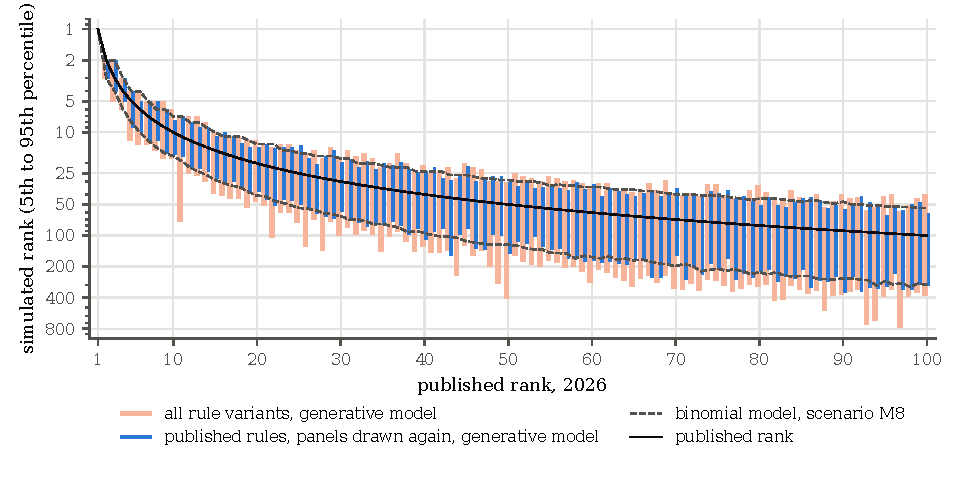
\includegraphics[width=\textwidth]{figures/fig_intervals.pdf}
\caption{Rank intervals for the 2026 top 100. Blue: 5th to 95th percentile over panels drawn again under the published rules, pooled over the six worlds. Light orange: the same over all rule variants. Dashed: the binomial model of Section~\ref{sec:scenarios}, scenario M8. The vertical axis is logarithmic.}
\label{fig:intervals}
\par\smallskip{\footnotesize Alt text: Vertical intervals of simulated rank for each of the 100 restaurants of the 2026 list, on a logarithmic axis. The intervals are a few places wide at the top and widen steadily down the list, spanning more than a hundred places in the lower half, and the binomial model gives similar widths.\par}
\end{figure}

Figure~\ref{fig:intervals} gives the interval for each restaurant of the 2026 list, and Table~\ref{tab:intervals} of the supplementary material lists them. The generative model and the binomial model agree closely on the width of the intervals under the published rules. Restaurants published at No.10, No.15 and No.25 have 90\% intervals of 8 to 16, 11 to 28 and 14 to 50. Le Coquillage, published at No.34, could have been anywhere from No.23 to No.78, and the restaurants published at No.50 and No.51 could each have been anywhere from the low 30s to well below No.100. Aggregates are no safer. Japan has no restaurant in the 2026 top 50, but its five restaurants published between No.52 and No.91 put at least one in the top 50 in 80\% of simulated editions under the published rules. Peru's three places in the top 50 become two in 43\% of editions. The model's certainty about No.1 and No.2 should not be read as a finding. It follows from the power-law curve, which separates the first positions by tens of votes, and the margin at the top is as unknown as the rest.

\section{What would make the list more auditable}\label{sec:remedies}

The main obstacle to an audit is not the design of the vote but the absence of the numbers that would allow its precision to be checked. Publishing the vote count of each listed restaurant, or bands of counts if exact figures are judged too sensitive, would settle most of the questions raised here. Publishing which positions are tied and how each tie was broken would show how much of the order is set by the secondary rule. Publishing rank intervals of the kind computed in Section~\ref{sec:scenarios} would show readers which differences mean something. A list presented in tiers below about the 25th position would claim no more than the vote supports. Describing the list as the restaurants most often named by a panel of travelling experts, rather than as the world's best, would align its presentation with what the vote measures.

The rules should be stated completely and in one place. This includes the number of voters per region, whether the ballot is fixed at ten votes, how the order of preference is used, and whether the normalisation of regional vote shares exists, what triggers it, what it does and in which editions it was applied. The adjudicator's procedures and their findings, such as the share of ballots whose proof of visit was checked, would turn a statement of integrity into evidence. Finally, ballot data released to researchers under a confidentiality agreement would allow a full audit, including of the effects of voter recruitment, constituency mix, travel and host destinations, none of which can be estimated from outside.

\section{Limitations}

The audit rests on the published lists and on models of the vote. The limits of Section~\ref{sec:bounds} do not depend on the vote curve but assume independent binomial counts. The fixed number of voters per region loosens them only slightly, while the positive association between restaurants named on the same trips, which cannot be measured from outside, would loosen them by an unknown amount. The vote curve is unknown, so the precision of Sections~\ref{sec:scenarios} and~\ref{sec:gsa} is reported over a range of curves that we constrained only by the observed churn, and a power law may misrepresent the head of the distribution. The binomial and Plackett--Luce models treat voters as independent and identical within regions. Correlated recruitment and shared travel would add noise, while persistent tastes of returning voters reduce year-on-year churn, which our two bounds bracket. The generative model's tail of unlisted restaurants is spread evenly over regions, and its home unit is the region, whereas the 2026 cap applies to countries, which loosens it in multi-country regions. The supply-based allocation is one of many alternatives. The normalisation step is not modelled because it is not defined. The organiser's archive of past lists departs from its own announcements at four positions, and the extended lists of 2019, 2021 and 2022 rest on press coverage checked against a second source. Several rules are documented only on versions of the organiser's pages from before the September 2026 rebrand, which now redirect and which we read in search-engine indexes. The repository includes a script that retrieves archived copies of these pages and adds them to the references.

\section{Conclusions}\label{sec:conclusions}

The audit supports six conclusions, which rest on the levels of evidence of Table~\ref{tab:evidence}. First, from the published lists alone, positions below the top ten move by a median of 9 to 18.5 places between editions, and since former winners were retired in 2019 the title has gone in six of seven editions to the highest-placed eligible restaurant of the year before. Second, under any distribution of votes, integer counts from at most 11,200 votes cannot order the lower half of the list. At most 12 of the 49 adjacent pairs between No.51 and No.100 could be kept in order by a fresh panel of independent voters with probability 0.95, and a list without ties there would need No.51 to have at least 49 more votes than No.100. Third, under the vote distributions consistent with the observed churn, most adjacent positions from No.51 to No.100 are tied, the year-on-year movements below the top 25 are of the size that the renewal of the panel alone produces, and a panel of the same size drawn again would put 10 to 12 different restaurants in the top 50. Fourth, in the generative model, the equal allocation of voters to regions shapes the geography of the list more than any other rule, the counting rule matters more than ballot length, the home-country cap or the tie-break, and Japan's absence from the 2026 top 50 would recur in only one simulated edition in five.

Fifth, what the list measures is how often a restaurant appears on the ballots of a travelling, partly self-selected panel. That is its visibility to that panel, which depends on where the voters live and travel, including to host destinations, as well as on the quality of its cooking. The rules that decide who votes therefore decide whose visits count. Sixth, the list cannot be audited from outside, because neither the vote counts nor the regional normalisation, the adjudicator's procedures or the recruitment of voters are disclosed. Table~\ref{tab:checklist} reads these findings against the seven rules of sensitivity auditing.

\begin{table}[t]
\caption{The voting system read against the seven rules of sensitivity auditing.}
\label{tab:checklist}
\small
\begin{tabularx}{\textwidth}{@{}P{3.6cm}L@{}}
\toprule
Rule & Finding \\
\midrule
1. Check against the rhetorical use of quantification & A strict order from 1 to 100 under the label ``best'' conveys a precision that the vote does not have (Sections~\ref{sec:noise} and~\ref{sec:gsa}). The organiser's own description of the list as a snapshot of opinions is not carried into its presentation. \\
2. Adopt an assumption-hunting attitude & Equal weight of 40 voters per region irrespective of the size of its dining scene; equal weight of every vote on a ballot; the home cap; the region map, set by the organiser and reviewed every year; the constituency mix of writers, chefs and gourmets; the retirement of winners. \\
3. Detect garbage in, garbage out & Vote counts are integers from at most 11,200 votes. The published order below No.25 is finer than the counts can support, and the order within ties comes from a secondary rule. \\
4. Find sensitive assumptions before they find you & The vote distribution and the panel draw dominate agreement with the published order, and the allocation of voters to regions dominates its geography. The counting rule matters more than ballot length, home cap or tie-break (Section~\ref{sec:gsa}). \\
5. Aim for transparency & No vote counts, ties, margins, regional vote shares or ballot data are published. The normalisation step and the adjudicator's procedures are undefined. Voter recruitment is delegated to Chairs who also advise on the brand. \\
6. Do the right sums & The question the list answers is how often a restaurant appears on the ballots of a travelling, partly self-selected panel. That is a measure of visibility among that panel as much as of quality, and it depends on where voters travel, including to host destinations. \\
7. Perform thorough uncertainty and sensitivity analysis & Not done by the organiser. Sections~\ref{sec:noise} and~\ref{sec:gsa} provide a first one. \\
\bottomrule
\end{tabularx}
\end{table}

The 50 Best Restaurants list is one instance of a common device: a ranking produced by the ballots of a panel and published as a strict order without the counts behind it. The audit shows what can be said about such a device from outside. The published rules and lists establish how unstable positions are and how the rules have changed. Arithmetic on integer counts and the variability of independent voters bound the precision of the order under any distribution of votes, which is the strongest kind of statement available while the votes are secret. Scenarios and a generative model of ballots then show which design choices matter, at the price of assumptions that the audit states. The same sequence applies to reputation surveys, critics' polls and awards decided by panels. Rankings of this kind would be easier to audit, and clearer about their meaning, if they published their counts and described themselves as what they are.

\section*{Data availability}

The lists, the code that assembles and checks them, and the analyses are available at \url{https://github.com/Confareneoclassico/50best-voting-audit} and archived on Zenodo \citep{lopiano2026code}. The published lists are in \texttt{data/raw}, with the organiser's archive in \texttt{data/raw/organiser\_archive} and the sources of every file, and the assembled panel of all editions is \texttt{data/derived/panel.csv}. \texttt{src/lists.py} builds the panel, \texttt{src/churn.py} the empirical part, \texttt{src/bounds.py} the limits under any vote curve, \texttt{src/noise.py} the binomial scenarios, \texttt{src/voting\_model.py} and \texttt{src/gsa.py} the generative model and the sensitivity analysis, and \texttt{tests/} holds the checks. These include the reproduction of every position of the organiser's archive with the four documented corrections, of the published 2023 changes and of the 2016 list with its 2015 ranks, analytic tests of the estimators, and an offline test of the archiving tool. \texttt{tools/archive\_sources.py} retrieves archived copies of the web sources, and \texttt{data/raw/archived\_sources.csv} lists the copies cited in the references.

\section*{Acknowledgements}

The author used Claude (Anthropic), a large language model, throughout this work: to write and test the code in the repository, to assemble and check the data, to search for and summarise sources, and to draft and revise the text. A separate instance of the model reviewed the code independently. The author directed the work, checked the code, data, sources and text, and takes full responsibility for the content. No specific funding was received for this work.

\bibliographystyle{plainnat}
\bibliography{refs}

\appendix
\section{Data assembly and checks}\label{app:data}

The lists of 2002 to 2025 come from the organiser's archive of past lists \citep{the50archive}, one page per edition, which gives positions 1 to 50 up to 2022 and 1 to 100 from 2023. We keep each edition as printed in \texttt{data/raw/organiser\_archive}. The archive departs from the organiser's announcements at the time in three editions. In 2016 it gives positions 22 and 23 twice and omits 18 and 37, which the organiser's 2016 list in pictures and the full list printed by The Atlanta Journal-Constitution with each restaurant's 2015 rank assign to White Rabbit and Nahm \citep{w50b2016pictures,ajc2016}. In 2015 it numbers Tickets 43, while the announcement placed Tickets and Borag\'o jointly at No.42 \citep{w50b2015pictures}. In 2025 it gives position 27 twice and omits 28, which the announcement assigns to Lasai \citep{w50b2025lists}. We correct the four entries in a separate file (\texttt{data/raw/corrections.csv}). After the correction, all 50 positions of 2016 and every 2015 rank printed for them agree with the panel. The extended lists of 2019 (positions 51 to 120), 2021 and 2022 are no longer on the organiser's site. They come from press coverage reproducing the organiser's releases \citep{inkl2019,upcoming2021,upcoming2022}, each checked entry by entry against a second source \citep{hotdinners2019,hotdinners2021,hotdinners2022}. The 2026 list comes from the organiser's pages \citep{the50list2026}. Restaurant names are matched across editions by a normalised identifier with explicit aliases for spelling variants and for restaurants printed under another name, such as Bras for Michel Bras, Cracco Peck for Ristorante Cracco, and Hotel de Paris in Monaco for its restaurant Le Louis XV. Each restaurant is assigned one country, that of the location the organiser prints for it (\texttt{data/raw/restaurant\_countries.csv}). The locations printed in the early editions of the archive are not reliable, for instance Troisgros appears in Ouches, in Paris and in Lyon in different editions, so they are not used to match restaurants. One entry remains uncertain. Il Pescatore, No.33 in 2002, which the archive places in Orlando, may be Dal Pescatore of Canneto sull'Oglio, No.35 in 2003, or a namesake, and is kept as a restaurant of its own. Merging the two would raise the rank correlation among the restaurants that stayed in the top 50 from 2002 to 2003 from 0.32 to 0.34 and would change no other result. Two names refer to different restaurants depending on the edition, Gaggan before and after its 2019 closure and Noma before and after its relocation \citep{sansom2021noma}. Every edition passes checks of complete positions with no ties other than the one published in 2015, and the published 2023 changes since 2022 \citep{upcoming2023} are reproduced for all 50 restaurants of the extended list. The assembled panel of all editions from 2002 to 2026 is written to \texttt{data/derived/panel.csv}.

\end{document}
